\section{Rappel de la problématique}

Ce projet consiste en l'étude et l'implémentation de l'article \textit{Minimum Snap Trajectory Generation and Control for Quadrotors} par Daniel Mellinger et Vijay Kumar \cite{Mellinger2011} qui propose un contrôleur et un générateur de trajectoires pour un véhicule aérien multirotor. Plus précisément, nous faisont une implémentation seulement de la partie génération de trajectoire par une méthode d'optimisation numérique.

Lors du suivi d'une trajectoire, une solution triviale est souvent utilisée qui consiste en l'interpolation en ligne droite entre chaque point de cheminement ou \textit{waypoint} (Mellinger utilise plutôt l'apellation \textit{keyframe}). Ceci est inneficace car la courbure infinie à chaque waypoint oblige le quadricoptère à s'arrêter avant de passer au prochain waypoint. Mellinger propose donc de modéliser une trajectoire optimale par un polynôme défini par parties entièrement lisse à travers les différents waypoints tout en satisfaisant des contraintes sur les vitesses et accélérations possibles du véhicule. Ce problème est résolu en le reécrivant en problème d'optimisation quadratique.

Tout dabord Mellinger démontre que la dynamique d'un quadricoptère a la propriété dêtre différentiellement plat. C'est-à-dire que les états et les entrées peuvent être exprimées par les sorties du système et leurs dérivées. Nous avons donc le vecteur de sorties plates
$$\sigma = [x, y, z, \psi]^T$$
où $r = [x, y, z]^T$ est la position du centre de masse dans le système de coordonnées du monde et $\psi$ l'angle de lacet. Rappelons nous que dans un repère main droite centré sur un corps rigide, l'axe $x$ pointe vers l'avant, $y$ vers la gauche et $z$ vers le haut. Les angles de rotation autour de ces axes sont le roulis (\textit{roll}), tangage (\textit{pitch}) et lacet (\textit{yaw}) respectivement. À fin de garder le projet simple, nous ne considérons pas les angles de roulis et de tangage dans le problème mais nous savons qu'il est possible de le faire pour exécuter des manoeuvres accrobatiques tel que voler à travers une fenêtre inclinée.

\begin{figure}[h]
	\centering
	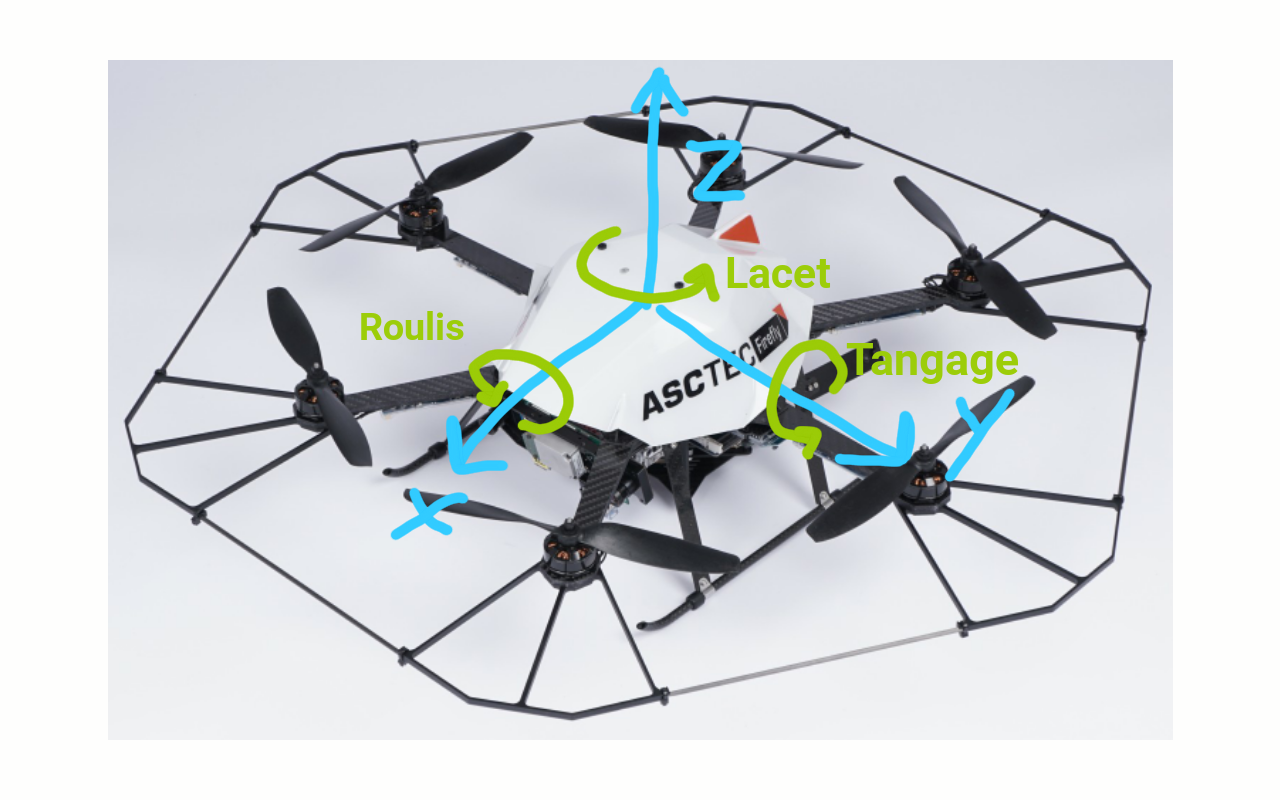
\includegraphics[width=0.5\textwidth]{fig/firefly.png}
	\caption{Systèmes de coordonnées d'un hexacoptère. L'angle de lacet est la rotation du véhicule autour de son axe Z, c'est-à-dire quand le véhicule tourne sur lui même.}
\end{figure}

Une trajectoire est définie comme était une courbe lisse dans l'espace des sorties plates:
$$ \sigma(t) : [t_0, t_m] \rightarrow \mathbb{R}^3 \times SO(2)$$
où $t_0$ et $t_m$ sont les temps de début et de fin de la trajectoire, $m$ correspond au nombre d'intervales de temps entre chaque waypoint et $SO(2)$ est le groupe spécial orthogonal. En pratique, une trajectoire est plutôt décrite par un polynôme défini par parties:
\begin{align}\label{eq:polynomial}
\sigma_T(t) =
\left\{
	\begin{array}{ll}
		\sum_{i=0}^n \sigma_{Ti1} t^i  & t_0 \leq t < t_1 \\
		\sum_{i=0}^n \sigma_{Ti2} t^i  & t_1 \leq t < t_2 \\
		... \\
		\sum_{i=0}^n \sigma_{Tim} t^i  & t_{m-1} \leq t < t_m \\
	\end{array}
\right.
\end{align}
où $n$ est l'ordre du polynôme et $m$ est encore le nombre d'intervales de temps.

Étant donné que l'on veut optimiser la dérivée d'ordre $k_r = 4$ (le \textit{snap}) de la position au carré et la dérivée d'ordre $k_\psi = 2$ (accélération angulaire) de langle de lacet $\psi$ au carré, nous avons le problème d'optimisation:
\begin{align}\label{eq:opt}
\text{min} \int_{t_0}^{t_m} \mu_r \norm{\frac{d^4 \boldsymbol{r}_T}{dt^4}}^2 + \mu_\psi {\ddot{\psi}_T}^2 dt
\end{align}\begin{align*}
	\begin{array}{lll}
%		\text{sous contraintes} & \sigma_T(t_i) = \sigma_i & i = 0, \ldots, m\\
		\text{sous contraintes} & \boldsymbol{r}_T(t_i) = \boldsymbol{r}_i & i = 0, \ldots, m\\
		& \psi_T(ti)=\psi_i & i = 0, \ldots, m\\
		& \frac{d^p x_T}{dt^p}|_{t=t_j} = 0\ \text{ou libre,} & j = 0, m; p = 1, 2, 3, 4\\
		& \frac{d^p y_T}{dt^p}|_{t=t_j} = 0\ \text{ou libre,} & j = 0, m; p = 1, 2, 3, 4\\
		& \frac{d^p z_T}{dt^p}|_{t=t_j} = 0\ \text{ou libre,} & j = 0, m; p = 1, 2, 3, 4\\
		& \frac{d^p \psi_T}{dt^p}|_{t=t_j} = 0\ \text{ou libre,} & j = 0, m; p = 1, 2\\
	\end{array}
\end{align*}

où $\boldsymbol{r}_T = [x_T, y_T, z_T]^T$ et $r_i = [x_i, y_i, z_i]$.
